%%22:47:26 19/10/2016 -VieTeX creates E:\tex\book-mau\mau-dethi30\cauhoi-toan-2017.tex
\baitracnghiem{t2017:b01}{%
Đường cong trong hình bên là đồ thị 
\begin{window}[0,r,{
\parbox[t]{0.3\linewidth}{\centering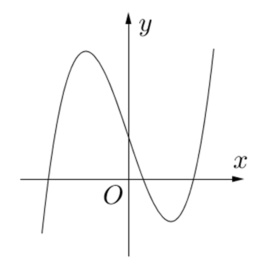
\includegraphics[scale=0.6]{toan01}}},{\label{fig:b01}}]
của một hàm số trong  bốn hàm số được liệt kê ở bốn phương án $A, B, C, D$ dưới
đây.  Hỏi hàm số đó là hàm số nào ?
\end{window}
}{
\datcot[2]
\bonpa
{\sai{$y=-x^2+x-1$.}}
{\sai{$y=-x^3+3x+1$.}}
{\dung{$y=x^3-3x+1$.}}
{\sai {$y=x^4-x^2+1$.}}
\loigiai{ 
Dựa vào đồ thị hàm số ta loại đi 2 đáp án A và C.\\
Dựa vào đồ thị hàm số ta suy ra bảng biến thiên của hàm số có dạng\\
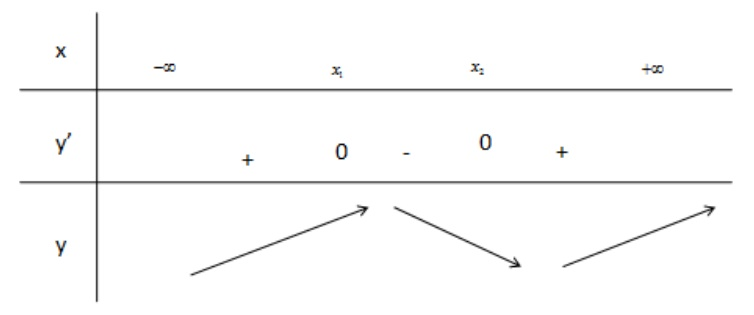
\includegraphics[scale=0.5]{gtoan01}\\
Như vậy ta thấy $y’ = 0$ có 2 nghiệm phân
 biệt và $y’$ trái dấu với hệ số của a nên hệ số $a > 0$
}
}

\baitracnghiem{t2017:b02}{%
Cho hàm số $y=f(x)$ có  $\lim\limits_{x\rightarrow +\infty}f(x)=1$ và   $\lim\limits_{x\rightarrow -\infty}f(x)=-1$. Khẳng định nào sau
đây là khẳng định đúng ?
}{
\datcot[2]
\bonpa
{\sai{Đồ thị hàm số đã cho không có tiệm cận ngang.}}
{\sai{Đồ thị hàm số đã cho có đúng một tiệm cận ngang.}}
{\dung{Đồ thị hàm số đã cho có hai tiệm cận ngang là các đường thẳng  $y=1$ và  $y=-1$.}}
{\sai{Đồ thị hàm số đã cho có hai tiệm cận ngang là các đường thẳng $x=1$ và  $x=-1$.}}
\loigiai{
Vì  $\lim\limits_{x\rightarrow\infty} f(x)=1$ nên hàm số có tiệm cận ngang $y = 1$\\
Vì  $\lim\limits_{x\rightarrow-\infty} f(x)=1$ nên hàm số có tiệm cận ngang $y =-1$\\
Vậy hàm số có 2 tiệm cận ngang.
}
}

\baitracnghiem{t2017:b03}{%
 Hỏi hàm số $y=2x^4+1$  đồng biến trên khoảng nào ?
}{
\datcot
\bonpa
{\sai{$\left(-\infty; -\dfrac{1}{2}\right)$.}}
{\dung{$\left(0;+\infty\right)$.}}
{\sai{$\left(-\dfrac{1}{2}; +\infty\right)$.}}
{\sai {$(-\infty;0)$.}}
\loigiai{
$y=2x^4+1\Rightarrow y'=8x^3$.\\
Với $x\in (0,\; +\infty)\Rightarrow y'>0 \Rightarrow $ Hàm số đồng biến trên $(0; +\infty)$
}
}

\baitracnghiem{t2017:b04}{%
Cho hàm số  $y=f(x)$ xác định, liên tục trên $\mathbb{R}$ và có bảng biến thiên :
\begin{center}
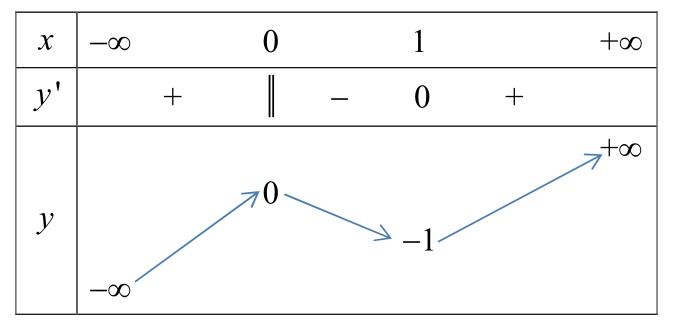
\includegraphics[scale =0.5]{toan02}
\end{center}
Khẳng định nào sau đây là khẳng định đúng ?
}{
\datcot[2]
\bonpa
{\sai{Hàm số có đúng một cực trị.}}
{\sai{Hàm số có giá trị cực tiểu bằng $1$.}}
{\sai {Hàm số có giá trị lớn nhất bằng $0$ và giá trị nhỏ nhất bằng  $1$.}}
{\dung{Hàm số đạt cực đại tại  $x=0$ và đạt cực tiểu tại  $x=1$.}}
\loigiai{Hàm số đạt cực đại tại  $x=0$ và đạt cực tiểu tại  $x=1$.
}
}

\baitracnghiem{t2017:b05}{%
Tìm giá trị cực đại $y_{\mbox{\scriptsize  \textit{CĐ} }}$ của hàm số $y=x^3-3x+2$.
}{
\datcot
\bonpa
{\dung{$y_{\mbox{\scriptsize \textit{CĐ} }}=4$.}}
{\sai{$y_{\mbox{\scriptsize \textit{CĐ} }}=1$.}}
{\sai{$y_{\mbox{\scriptsize  \textit{CĐ} }}=0$.}}
{\sai {$y_{\mbox{\scriptsize \textit{CĐ} }}=-1$.}}
\loigiai{
Ta có $y=x^3-3x+2$; $y'=3x^2-3$; $y'=0 \Leftrightarrow x=\pm 1$.\\
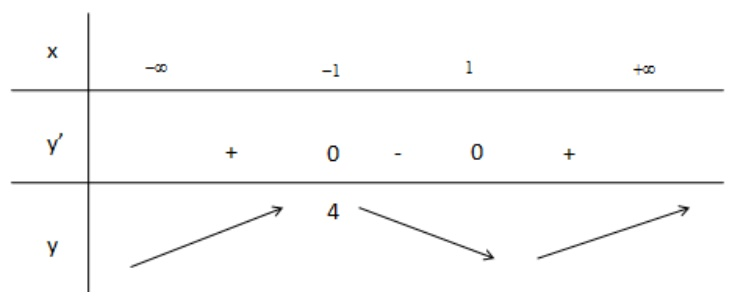
\includegraphics[scale=0.5]{gtoan02}\\
}
}

\baitracnghiem{t2017:b06}{%
Tìm giá trị nhỏ nhất của hàm số $y=\dfrac{x^2+3}{x-1}$ trên đoạn $[2;4]$.
}{
\datcot
\bonpa
{\dung{$\min_{[2;4]} y=6$.}}
{\sai{$\min_{[2;4]} y=-2$.}}
{\sai{$\min_{[2;4]} y=-3$.}}
{\sai {$\min_{[2;4]} y=\dfrac{19}{3}$.}}
\loigiai{
\begin{align*}
y&=\dfrac{x^2+3}{x-1}.\\
y'&=\dfrac{2x(x-1)-x^2-3}{(x-1)^2}=\dfrac{x^2-2x-3}{(x-1)^2}.\\
y'&=0\Leftrightarrow\left[\begin{matrix}
x=-1\quad \mbox{ loại }\\ 
x=3\quad \mbox{ thỏa mãn }\\ 
\end{matrix}\right..
\end{align*}
Có $y(2)=7; y(3)=6; y(4)=\dfrac{19}{3} \Rightarrow \min\limits_{[2;4]} y=6$.
}
}

\baitracnghiem{t2017:b07}{%
Biết rằng đường thẳng  $y=-2x+2$ cắt đồ thị hàm số
$y=x^3+x+2$ tại điểm
duy nhất; kí hiệu
$(x_0;y_0)$ là tọa độ của điểm đó. Tìm $y_0$.
}{
\datcot
\bonpa
{\sai{$y_0=4$.}}
{\sai{$y_0=0$.}}
{\dung{$y_0=2$.}}
{\sai {$y_0=-1$.}}
\loigiai{
Phương trình hoành độ giao điểm của đường thẳng và đồ thị hàm số là:\\
$x^3+x+2=-2x+2\Leftrightarrow x^3+3x=0 \Leftrightarrow x=0$\\
$y(0)=2$. 
}
}

\baitracnghiem{t2017:b08}{%
Tìm tất cả các giá trị thực của tham số $m$ sao cho đồ thị của hàm số $y=x^4+2mx^2+1$ có ba điểm cực trị tạo thành một tam giác vuông cân.
}{
\datcot
\bonpa
{\sai{$m=-\dfrac{1}{\sqrt[3]{9}}$.}}
{\dung{$m=-1$.}}
{\sai{$m=\dfrac{1}{\sqrt[3]{9}}$.}}
{\sai {$m=1$.}}
\loigiai{
$y=x^4+2mx^2+1$; $y'=4x^3+4mx$; $y'=0\Leftrightarrow 4x(x^2+m)=0 \Leftrightarrow
\left[\begin{matrix}
x=0;\\ 
x^2=-m\\ 
\end{matrix}\right.
$\\
Dựa vào đây ta thấy m phải là 1 giá trị nhỏ hơn 0 nên ta loại đi đáp án C và D.\\
Thử với đáp án B: với $m = -1$ ta có $y’ = 0$ có 3 nghiệm $x = 0; x = -1; x = 1$\\
$y(0)= 1; y (-1) = 0; y(1) = 0$\\
$\Rightarrow $ 3 điểm cực trị của là: $A(0;1); B(-1;0); C(1;0)$.\\
Ta thử lại bằng cách vẽ 3 điểm A, B, C trên cùng hệ trục tọa độ và tam giác này vuông cân.
}
}

\baitracnghiem{t2017:b09}{%
Tìm tất cả các giá trị thực của tham số m sao cho đồ thị của hàm số $y=\dfrac{x+1}{\sqrt{m x^2+1}}$
}{
\datcot[2]
\bonpa
{\sai{Không có giá trị thực nào của m thỏa mãn yêu cầu đề bài.}}
{\sai{$m<0$.}}
{\sai {$m=0$.}}
{\dung{$m>0$.}}
\loigiai{
Để hàm số có 2 tiệm cận ngang thì phải tồn tại $\lim\limits_{x\rightarrow +\infty} y\ne \lim\limits_{x\rightarrow -\infty}y$.\\
$\lim\limits_{x\rightarrow +\infty}y=\lim\limits_{x\rightarrow +\infty}\dfrac{x+1}{\sqrt{mx^2+1}}=\lim\limits_{x\rightarrow +\infty}\dfrac{1+\dfrac{1}{x}}{\sqrt{m+\dfrac{1}{x^2}}}=\dfrac{1}{\sqrt{m}}$,  tồn tại khi $m > 0$\\
Có $\lim\limits_{x\rightarrow +\infty}y=\lim\limits_{x\rightarrow +\infty}\dfrac{x+1}{\sqrt{mx^2+1}}=\lim\limits_{x\rightarrow +\infty}\dfrac{1+\dfrac{1}{x}}{-\sqrt{m+\dfrac{1}{x^2}}}=-\dfrac{1}{\sqrt{m}}$,  tồn tại khi $m > 0$\\
Khi đó hiển nhiên $\lim\limits_{x\rightarrow +\infty} y\ne \lim\limits_{x\rightarrow -\infty}y$.Vậy $m > 0$.
}
}

\baitracnghiem{t2017:b10}{%
Cho một tấm nhôm hình vuông cạnh 12 cm. 
% \begin{window}[0,r,{
% \parbox[t]{\linewidth/2}{\centering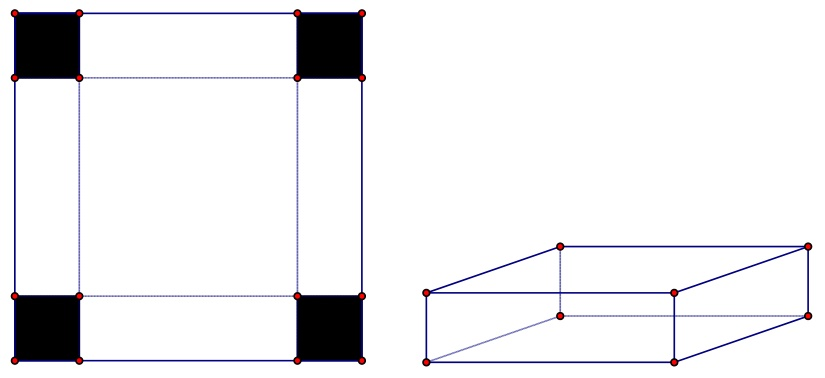
\includegraphics[scale =0.4]{toan03}}},{\label{fig:b31}}]
Người ta cắt ở bốn góc của tấm
nhôm đó bốn hình vuông bằng nhau, mỗi hình vuông có cạnh bằng $x$ (cm), rồi gập tấm
nhôm lại như hình vẽ dưới đây để được một cái hộp không nắp. Tìm $x$ để hộp nhận
được có thể tích lớn nhất.
% \end{window}
\begin{center}
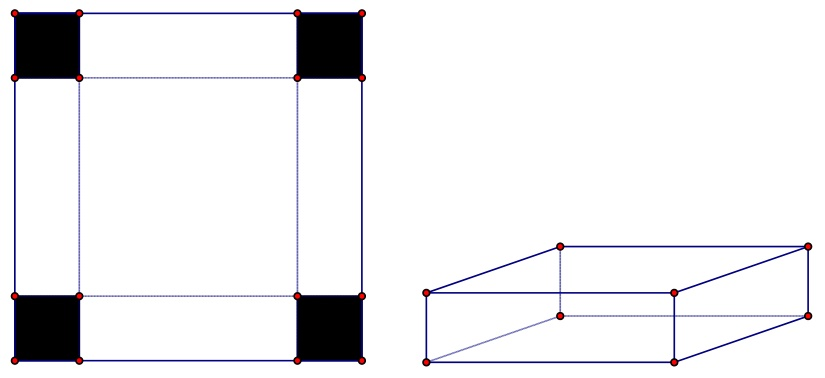
\includegraphics[scale =0.4]{toan03}
\end{center}
}{
\datcot
\bonpa
{\sai{$x=6$.}}
{\dung{$x=3$.}}
{\sai{$x=2$.}}
{\sai {$x=4$.}}
\loigiai{
Thể tích của hộp là
$$(12-2x)^2=\dfrac{1}{4}.4x(12-2x)^2\le \dfrac{1}{4}.\dfrac{(4x+12-2x+12-2x)^3}{27}=128.$$
Dấu bằng xảy ra khi  $4x=12-2x\Leftrightarrow x=2$.
Vậy x = 2 thì thể tích hộp lớn nhất.
}
}

\baitracnghiem{t2017:b11}{%
Tìm tất cả các giá trị thực của tham số $m$ sao cho hàm số $y=\dfrac{\tan x-2}{\tan x -m}$ đồng biến trên khoảng $\left(0;\dfrac{\pi}{4}\right)$.
}{
\datcot[2]
\bonpa
{\dung{$m\le 0$ hoặc $1\le m <2$.}}
{\sai{$m\le 0$.}}
{\sai{$\le m < 2$.}}
{\sai {$m\ge 2$.}}
\loigiai{
$$y'=\dfrac{\dfrac{1}{\cos^2x}(\tan x-m)-\dfrac{1}{\cos^2x}(\tan x-2)}{(\tan x-m)^2}=\dfrac{2-m}{\cos^2x(\tan x-m)^2}.$$
Hàm số đồng biến trên $\left(0;\dfrac{\pi}{4}\right)$ khi và chỉ khi hàm số xác định trên $\left(0;\dfrac{\pi}{4}\right)$ và $y'\ge 0$ $\forall x\in \left(0;\dfrac{\pi}{4}\right)$\\
$\Leftrightarrow \begin{cases}
\tan x\ne m,&\forall x\in \left(0;\dfrac{\pi}{4}\right)\\
2-m\ge 0&
\end{cases}\Leftrightarrow \left[\begin{matrix}
m\le 0\\ 
1\le m \le 2.\\ 
\end{matrix}\right.$.
}
}

\baitracnghiem{t2017:b12}{%
Giải phương trình $\log_4(x-1)=3$.
}{
\datcot
\bonpa
{\sai{$x=63$.}}
{\dung{$x=65$.}}
{\sai{$x=80$.}}
{\sai {$x=82$.}}
\loigiai{ 
Điện $x>1$.\\
Phương trình $\Leftrightarrow x-1=64\Leftrightarrow x=65$.
}
}

\baitracnghiem{t2017:b13}{%
Tính đạo hàm của hàm số $y=13^x$.
}{
\datcot
\bonpa
{\sai{$y'=x.13^{x-1}$.}}
{\dung{$y'=13^{x}.\ln 13$.}}
{\sai{$y'=13^{x}$.}}
{\sai {$y'=\dfrac{13^{x}}{\ln 13}$.}}
\loigiai{
 $y'=13^x.\ln 13$.
}
}

\baitracnghiem{t2017:b14}{%
Giải bất phương trình $\log_2(3x-1)>3$.
}{
\datcot
\bonpa
{\dung{$x>3$.}}
{\sai{$\dfrac{1}{3}<x<3$.}}
{\sai{$x<3$.}}
{\sai {$x>\dfrac{10}{3}$.}}
\loigiai{
Điều kiện: $x>\dfrac{1}{3}$. BPT $\Leftrightarrow 3x-1>8\Leftrightarrow x>3$.
Kết hợp điều kiện ta được $x > 3$.
}
}

\baitracnghiem{t2017:b15}{%
Tìm tập xác định $\mathcal{D}$ của hàm số $y=\log_2(x^2-2x-3)$.
}{
\datcot[2]
\bonpa
{\sai{$\mathcal{D}=(-\infty;-1]\cup [3;+\infty)$.}}
{\sai{$\mathcal{D}=[-1;3]$.}}
{\dung{$\mathcal{D}=(-\infty;-1)\cup (3;+\infty)$.}}
{\sai {$\mathcal{D}=(-1;3)$.}}
\loigiai{
$x^2-2x-3>0\Leftrightarrow x\in (-\infty;-1)\cup (3;+\infty)$. 
}
}

\baitracnghiem{t2017:b16}{%
Cho hàm số $f(x)=2^x.7^x$. Khẳng định nào sau đây là khẳng định \textbf{sai }?
}{
\datcot[2]
\bonpa
{\sai{$f(x)<1\Leftrightarrow  x+x^2\log_2 7<0$.}}
{\sai{$f(x)<1\Leftrightarrow  x\ln 2+x^2\ln 7<0$.}}
{\sai {$f(x)<1\Leftrightarrow  x\log_7 2+x^2<0$.}}
{\dung{$f(x)<1\Leftrightarrow  1+x\log_2 7<0$.}}
\loigiai{
$f(x)<1\Leftrightarrow 2^x.7^{x^2}<1\Leftrightarrow 7^{x^2}<2^{-x}\Leftrightarrow x^2.\ln 7<-x.\ln 2\Leftrightarrow x\ln 2+x^2\ln 7<0$\\
$\Leftrightarrow x+x^2\log_2 7<0\Leftrightarrow x\log_7 2+x^2<0$. 
}
}

\baitracnghiem{t2017:b17}{%
Cho các số thực dương $a, b,$ với $a\ne 1 $Khẳng định nào sau đây là khẳng định
đúng ?
}{
\datcot[2]
\bonpa
{\sai{$\log_{a^2}(ab)=\dfrac{1}{2}\log_a b$.}}
{\sai{$\log_{a^2}(ab)=2+2\log_a b$.}}
{\sai {$\log_{a^2}(ab)=\dfrac{1}{4}\log_a b$.}}
{\dung{$\log_{a^2}(ab)=\dfrac{1}{2}+\dfrac{1}{2}\log_a b$.}}
\loigiai{
$\log_{a^2}(ab)=\dfrac{1}{2}\log_a(ab)=\dfrac{1}{2}(1+\log_a b)=\dfrac{1}{2}+\dfrac{1}{2}\log_ab$.
}
}

\baitracnghiem{t2017:b18}{%
Tính đạo hàm của hàm số $y=\dfrac{x+1}{4^x}$.
}{
\datcot[2]
\bonpa
{\dung{$y'=\dfrac{1-2(x+1)\ln 2}{2^{2x}}$.}}
{\sai{$y'=\dfrac{1+2(x+1)\ln 2}{2^{2x}}$.}}
{\sai{$y'=\dfrac{1-2(x+1)\ln 2}{2^{x^2}}$.}}
{\sai {$y'=\dfrac{1+2(x+1)\ln 2}{2^{x^2}}$.}}
\loigiai{
$y=\dfrac{x+1}{4^x}$\\
$y'=\dfrac{4^x-4^x.(x+1)\ln 4}{4^{2x}}=\dfrac{1-2(x+1)\ln 2}{2^{2x}}$.
}
}

\baitracnghiem{t2017:b19}{%
Đặt $a=\log_2 3, b=\log_5 3$. Hãy biểu diễn $\log_6 45$ theo $a$ và $b$.
}{
\datcot[2]
\bonpa
{\sai{$\log_6 45=\dfrac{a+2ab}{ab}$.}}
{\sai {$\log_6 45=\dfrac{2a^2-2ab}{ab}$.}}
{\dung{$\log_6 45=\dfrac{a+2ab}{ab+b}$.}}
{\sai {$\log_6 45=\dfrac{2a^2-2ab}{ab+b}$.}}
\loigiai{
$\log_645\dfrac{\log_345}{\log_36}=\dfrac{\log_3(3^2.5)}{\log_3(2.3)}=\dfrac{2+\log_35}{1+\log_32}=\dfrac{2+\dfrac{1}{b}}{1+\dfrac{1}{b}}=\dfrac{2ab+a}{ab+b}$. 
}
}

\baitracnghiem{t2017:b20}{%
Cho hai số thực $a$ và $b$, với $1<a<b$.  Khẳng định nào dưới đây là khẳng định
đúng ?
}{
\datcot[2]
\bonpa
{\sai {$\log_a b<1<\log_b a$.}}
{\sai {$1<\log_a b<\log_b a$.}}
{\sai {$\log_b a<\log_a b<1$.}}
{\dung{$\log_b a<1<\log_a b$.}}
\loigiai{
$\log_b a<1<\log_a b$.
}
}

\baitracnghiem{t2017:b21}{%
Ông A vay ngắn hạn ngân hàng 100 triệu đồng, với lãi suất 12\%/năm. Ông
muốn hoàn nợ cho ngân hàng theo cách : Sau đúng một tháng kể từ ngày vay, ông bắt
đầu hoàn nợ; hai lần hoàn nợ liên tiếp cách nhau đúng một tháng, số tiền hoàn nợ ở mỗi
lần là như nhau và trả hết tiền nợ sau đúng 3 tháng kể từ ngày vay. Hỏi, theo cách đó, số
tiền $m$ mà ông A sẽ phải trả cho ngân hàng trong mỗi lần hoàn nợ là bao nhiêu ? Biết
rằng, lãi suất ngân hàng không thay đổi trong thời gian ông A hoàn nợ.
}{
\datcot[2]
\bonpa
{\sai {$m=\dfrac{100.(1,01)^3}{3}$ (triệu đồng).}}
{\dung{$m=\dfrac{(1,01)^3}{(1,01)^3-1}$ (triệu đồng).}}
{\sai {$m=\dfrac{100\times1,03}{3}$ (triệu đồng).}}
{\sai {$m=\dfrac{120.(1,12)^3}{(1,12)^3-1}$ (triệu đồng).}}
\loigiai{
Lãi suất 12\% / năm = 1\% / tháng (do vay ngắn hạn).\\
Sau tháng 1, ông A còn nợ  $100.1,01 - m$  (triệu).\\
Sau tháng 2, ông còn nợ  $(100.1,01-m).1,01-m=100.1,01^2-2,01m$ (triệu).\\
Sau tháng 3, ông hết nợ do đó\\
$(100.1,01^2-2,01m).1,01-m=100.1,01^3-3,0301m=0\Rightarrow m=\dfrac{100.1,01^3}{3,0301}=\dfrac{1,01^3}{1,01^3-1}$ (triệu đồng). 
}
}

\baitracnghiem{t2017:b22}{%
Viết công thức tính thể tích $V$ của khối tròn xoay được tạo ra khi quay hình
thang cong, giới hạn bởi đồ thị hàm số $y=f(x)$, trục $Ox$ và hai đường thẳng $x = a, x = b
(a < b)$, xung quanh trục $Ox$.
}{
\datcot[2]
\bonpa
{\dung{$V=\pi\int\limits_a^bf^2(x)dx$.}}
{\sai {$V=\int\limits_a^bf^2(x)dx$.}}
{\sai {$V=\pi\int\limits_a^bf(x)dx$.}}
{\sai {$V=\pi\int\limits_a^b|f(x)|dx$.}}
\loigiai{
$V=\pi\int\limits_a^bf^2(x)dx$.
}
}

\baitracnghiem{t2017:b23}{%
Tìm nguyên hàm của hàm số $f(x)=\sqrt{2x-1}$.
}{
\datcot[2]
\bonpa
{\sai {$\int f(x)dx=\dfrac{2}{3}(2x-1)\sqrt{2x-1}+C$.}}
{\dung{$\int f(x)dx=\dfrac{1}{3}(2x-1)\sqrt{2x-1}+C$.}}
{\sai {$\int f(x)dx=-\dfrac{1}{3}(2x-1)\sqrt{2x-1}+C$.}}
{\sai {$\int f(x)dx=\dfrac{1}{2}(2x-1)\sqrt{2x-1}+C$.}}
\loigiai{
$\int\sqrt{2x-1}dx=\dfrac{1}{2}\int(2x-1)^{\tfrac{1}{2}}d(2x-1)=\dfrac{1}{2}.\dfrac{(2x-1)^{\tfrac{3}{2}}}{\dfrac{3}{2}}+C=\dfrac{1}{3}(2x-1)\sqrt{2x-1}+c $. 
}
}

\baitracnghiem{t2017:b24}{%
 Một ô tô đang chạy với vận tốc 10m/s thì người lái đạp phanh; từ thời điểm đó, ô
tô chuyển động chậm dần đều với vận tốc  $v(t)=-5t+10$(m/s), trong đó $t$ là khoảng thời
gian tính bằng giây, kể từ lúc bắt đầu đạp phanh. Hỏi từ lúc đạp phanh đến khi dừng hẳn, ô
tô còn di chuyển bao nhiêu mét ?
}{
\datcot
\bonpa
{\sai {0,2m.}}
{\sai {2m.}}
{\dung{10m.}}
{\sai {20m.}}
\loigiai{
Ô tô còn đi thêm được 2 giây. \\
Quãng đường cần tìm là $s=\int\limits_0^2 v(t)dt=\int\limits_0^2(-5t+10)dt=\left(-\dfrac{5t^2}{2}+10t\right)\big|_0^2=10(m)$. 
}
}

\baitracnghiem{t2017:b25}{%
 Tính tích phân $I=\int\limits_0^{\pi}\cos^3 x. \sin x dx$.
}{
\datcot
\bonpa
{\sai {$I=-\dfrac{1}{4}\pi^4$.}}
{\sai {$I=-\pi^4$.}}
{\dung{$I=0$.}}
{\sai {$I=-\dfrac{1}{4}$.}}
\loigiai{
Sử dụng máy tính. I = 0. 
}   
}

\baitracnghiem{t2017:b26}{%
Tính tích phân $I=\int\limits_1^e x\ln x dx$
}{
\datcot
\bonpa
{\sai {$I=\dfrac{1}{2}$.}}
{\sai {$I=\dfrac{e^2-2}{2}$.}}
{\dung{$I=\dfrac{e^2+1}{4}$.}}
{\sai {$I=\dfrac{e^2-1}{4}$.}}
\loigiai{
Dùng máy tính kiểm tra từng đáp án hoặc.\\
$u=\ln x, dv=xdx\Rightarrow du=\dfrac{dx}{x}, v=\dfrac{x^2}{2}$.\\
$I=\dfrac{x^2\ln x}{2}\bigg|_1^e-\int\limits_1^e\dfrac{x}{2}dx=\dfrac{e^2}{2}-\left(\dfrac{e^2}{4}-\dfrac{1}{4}\right)=\dfrac{e^2+1}{2}$.
}  
}

\baitracnghiem{t2017:b27}{%
Tính diện tích hình phẳng giới hạn bởi đồ thị hàm số $y=x^3-x$ và đồ thị hàm
số $y=x-x^2$.
}{
\datcot
\bonpa
{\dung{$\dfrac{37}{12}$.}}
{\sai {$\dfrac{9}{4}$.}}
{\sai {$\dfrac{81}{12}$.}}
{\sai {$13$.}}
\loigiai{
Xét phương trình hoành độ giao điểm\\
 $x^3-x=x-x^2\Leftrightarrow x^3+x^2-2x=0\Leftrightarrow\left[\begin{matrix}
x=-2\\ 
x=0\\ 
x=1\\ 
\end{matrix}\right.$.\\
Diện tích cần tính:\\
$S=\int\limits_{-2}^1|x^3-x-x+x^2|dx=\int \limits_{-2}^0(x^3+x^2-2x)dx+\int \limits_0^1(-x^3-x^2+2x)dx=\dfrac{8}{3}+\dfrac{5}{12}=\dfrac{37}{12}$.
}  
}

\baitracnghiem{t2017:b28}{%
Kí hiệu $(H)$ là hình phẳng giới hạn bởi đồ thị hàm số  $y=2(x-1)e^x$, trục tung
và trục hoành. Tính thể tích $V$ của khối tròn xoay thu được khi quay hình $(H)$ xung
quanh trục $Ox$.
}{
\datcot
\bonpa
{\sai {$V=4-2e$.}}
{\sai {$V=(4-2e)\pi$.}}
{\sai {$V=e^2-5$.}}
{\dung{$V=(e^2-5)\pi$.}}
\loigiai{
Xét giao điểm $2(x-1)e^x=0\Leftrightarrow x=1$. Thể tích cần tính:\\
$V=\pi\int \limits  _0^1\left[2(x-1)e^x\right]^2dx=4\pi\int \limits_0^1 (x-1)^2e^{2x}dx=\pi(e^2-5)$ (dùng máy tính thử). 
}  
}

\baitracnghiem{t2017:b29}{%
Cho số phức  $z=3-2i$. Tìm phần thực và phần ảo của số phức $\bar z$
}{
\datcot[2]
\bonpa
{\sai {Phần thực bằng $-3$ và Phần ảo bằng $-2i$.}}
{\sai {Phần thực bằng $-3$ và Phần ảo bằng $-2$.}}
{\sai {Phần thực bằng $3$ và Phần ảo bằng $2i$.}}
{\dung{Phần thực bằng $3$ và Phần ảo bằng $2$.}}
\loigiai{
Số phức liên hợp của $z$ là $3 + 2i$, phần thực 3, phần ảo 2.
}  
}

\baitracnghiem{t2017:b30}{%
 Cho hai số phức $z_1=1+i$ và $z_2=2-3i$. Tính môđun của số phức $z_1+z_2$
}{
\datcot
\bonpa
{\dung{$|z_1+z_2|=\sqrt{13}$.}}
{\sai {$|z_1+z_2|=\sqrt{5}$.}}
{\sai {$|z_1+z_2|=1$.}}
{\sai {$|z_1+z_2|=5$.}}
\loigiai{
$z_1+z_2=3-2i\Rightarrow |z_1+z_2|=\sqrt{3^2+(-2)^2}=\sqrt{13}$. 
}  
}

\baitracnghiem{t2017:b31}{%
Cho số phức $z$ thỏa mãn $(1+i)z=3-i$ . 
\begin{window}[0,r,{
\parbox[t]{0.3\linewidth}{\centering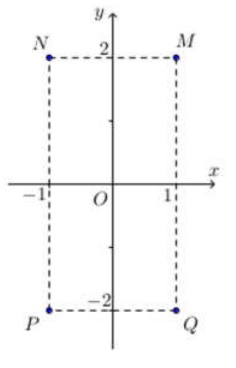
\includegraphics[scale=0.6]{toan04}}},{\label{fig:b31}}]
Hỏi điểm biểu
diễn của z là điểm nào trong các điểm $M, N, P, Q$ ở hình bên ?
\end{window}
}{
%  \setlength{\shortitemwidth}{0.34\linewidth}
\datcot[4]
\bonpa
{\sai {Điểm $P$.}}
{\dung{Điểm $Q$.}}
{\sai {Điểm $M$.}}
{\sai {Điểm $N$.}}
% \end{multicols}
\loigiai{
$(1+i)z=3-i\Rightarrow z=\dfrac{3-i}{1+i}=1-2i\Rightarrow Q(1;-2)$ là điểm biểu diễn $z$. 
}  
}

\baitracnghiem{t2017:b32}{%
Cho số phức  $z=2+5i$. Tìm số phức  $w=iz+\overline{z}$ .
}{
\datcot
\bonpa
{\sai {$w=7-3i$.}}
{\dung{$w=-3-3i$.}}
{\sai {$w=3+7i$.}}
{\sai {$w=-7-7i$.}}
\loigiai{
$\bar z=2-5i\Rightarrow w=i(2+5i)+2-5i=-3-3i$.
}  
}

\baitracnghiem{t2017:b33}{%
Kí hiệu $z_1, z_2, z_3$ và $z_4$ là bốn nghiệm phức của phương trình $z^4-z^2-12=0$.
Tính tổng $T=|z_1|+|z_2|+|z_3|+|z_4|$. 
}{
\datcot
\bonpa
{\sai {$T=4$.}}
{\sai {$T=2\sqrt3$.}}
{\dung{$4+2\sqrt3$.}}
{\sai {$T=2+2\sqrt3$.}}
\loigiai{
$z^4-z^2-12=0\Leftrightarrow (z^2-4)(z^2+3)=0\Leftrightarrow \left[\begin{matrix}
z=\pm 2\\ 
z=\pm i\sqrt3\\ 
\end{matrix}\right.$.\\
 $\Rightarrow T=2+2+\sqrt3+\sqrt3=4+2\sqrt3$. 
}  
}

\baitracnghiem{t2017:b34}{%
Cho các số phức $z$ thỏa mãn$ | z | = 4$. Biết rằng tập hợp các điểm biểu diễn các
số phức  $w=(3+4i)z+i$ là một đường tròn. Tính bán kính $r$ của đường tròn đó.
}{
\datcot
\bonpa
{\sai {$r=4$.}}
{\sai {$r=5$.}}
{\dung{$r=20$.}}
{\sai {$r=22$.}}
\loigiai{
$w=x+yi\quad (x,y\in\mathbb{R})\Rightarrow z=\dfrac{w-i}{3+4i}=\dfrac{x+(y-1)i}{3+4i}=\dfrac{3x-4(y-1)+[3(y-1)+4x]}{25}$.\\
$16=|z|^2=\left(\dfrac{3x-4y+4}{25}\right)^2+\left(\dfrac{4x+3y-3}{25}\right)\Rightarrow x^2+(y-1)^2=400\Rightarrow r=20$.
}  
}

\baitracnghiem{t2017:b35}{%
Tính thể tích $V$ của khối lập phương  $ABCD. A' B' C' D'$ , biết  $AC=a\sqrt3$.
}{
\datcot
\bonpa
{\dung{$V=a^3$.}}
{\sai {$V=\dfrac{3\sqrt6a^3}{4}$.}}
{\sai {$V=3\sqrt3a^3$.}}
{\sai {$V=\dfrac{1}{3}a^3$.}}
\loigiai{
Cạnh của hình lập phương là $\dfrac{AC'}{\sqrt3}=a \Rightarrow$ Thể tích $V=a^3$.
}  
}

\baitracnghiem{t2017:b36}{%
Cho hình chóp tứ giác $S.ABCD$ có đáy $ABCD$ là hình vuông cạnh a, cạnh bên
$SA$ vuông góc với mặt phẳng đáy và  $SA=\sqrt2 a$. Tính thể tích $V$ của khối chóp $S.ABCD$.
}{
\datcot
\bonpa
{\sai {$V=\dfrac{\sqrt2 a^3}{6}$.}}
{\sai {$V=\dfrac{\sqrt2 a^3}{4}$.}}
{\sai {$V=\sqrt2 a^3$.}}
{\dung{$V=\dfrac{\sqrt2 a^3}{3}$.}}
\loigiai{
$V=\dfrac{1}{3}SA.S_{ABCD}=\dfrac{1}{3}a\sqrt2 a^2=\dfrac{\sqrt2 a^3}{3}$. 
}  
}

\baitracnghiem{t2017:b37}{%
 Cho tứ diện $ABCD$ có các cạnh $AB, AC$ và $AD$ đôi một vuông góc với nhau; $AB = 6a$,
$AC = 7a$ và $AD = 4a$. Gọi $M, N, P$ tương ứng là trung điểm các cạnh $BC, CD, DB$. Tính thể tích
$V$ của tứ diện $AMNP$.
}{
\datcot
\bonpa
{\sai {$V=\dfrac{7}{2}a^3$.}}
{\sai {$V=14a^3$.}}
{\sai {$V=\dfrac{28}{3}a^3$.}}
{\dung{$V=7a^3$.}}
\loigiai{
$V_{ABCD}=\dfrac{1}{6}AB.AC.AD=28a^3\Rightarrow V_{AMNP}=\dfrac{1}{4}V_{ABCD}=7a^3$. 
}  
}

\baitracnghiem{t2017:b38}{%
Cho hình chóp tứ giác $S.ABCD$ có đáy là hình vuông cạnh bằng $\sqrt2a $. Tam
giác $SAD$ cân tại $S$ và mặt bên $(SAD)$ vuông góc với mặt phẳng đáy. Biết thể tích khối
chóp $S.ABCD$ bằng $\dfrac{4}{3}a^3$. Tính khoảng cách h từ B đến mặt phẳng (SCD).
}{
\datcot
\bonpa
{\sai {$h=\dfrac{2}{3}a$.}}
{\dung{$h=\dfrac{4}{3}a$.}}
{\sai {$h=\dfrac{8}{3}a$.}}
{\sai {$h=\dfrac{3}{4}a$.}}
\loigiai{
Gọi $H$ là trung điểm $AD\Rightarrow SH\perp (ABCD)$. Có $HS=\dfrac{3V_{S.ABCD}}{S_{ABCD}}=\dfrac{4a^3}{(\sqrt2 a)^2}$.\\
Vẽ $HK\perp SD$ tại $K\Rightarrow HK\perp (SCD)$\\
$AB//(SCD)\Rightarrow d=d(B;(SCD))=d(A;(SCD))=2d(H;(SCD))=2HK$.\\
Có $\dfrac{1}{HK^2}=\dfrac{1}{HS^2}+\dfrac{1}{HD^2}\Rightarrow HK=\dfrac{2}{3}a\Rightarrow d=\dfrac{4}{3}a$. 
}  
}

\baitracnghiem{t2017:b39}{%
Trong không gian, cho tam giác $ABC$ vuông tại $A, AB = a$ và   $AC=\sqrt3 a$. Tính
độ dài đường sinh l của hình nón, nhận được khi quay tam giác $ABC$ xung quanh trục $AB$.
}{
\datcot
\bonpa
{\sai {$l=a$.}}
{\sai {$l=\sqrt2a$.}}
{\sai {$l=\sqrt3a$.}}
{\dung{$l=2a$.}}
\loigiai{
Đường sinh của hình nón có độ dài bằng đoạn $BC=\sqrt{AB^2+AC^2}=2a$.
}  
}

\baitracnghiem{t2017:b40}{%
Từ một tấm tôn hình chữ nhật kích thước 50cm $\times$ 240cm, người ta làm các
thùng đựng nước hình trụ có chiều cao bằng 50cm, theo hai cách sau (xem hình minh
họa dưới đây) :
\begin{itemize}
\item 
 Cách 1 : Gò tấm tôn ban đầu thành mặt xung quanh của thùng.
\item 
 Cách 2 : Cắt tấm tôn ban đầu thành hai tấm bằng nhau, rồi gò mỗi tấm đó thành mặt
xung quanh của một thùng.
\end{itemize}
Kí hiệu $V_1$ là thể tích của thùng gò được theo cách 1 và
$V_2$ là tổng thể tích của hai thùng
gò được theo cách 2. Tính tỉ số $\dfrac{V_1}{V_2}$.
\begin{center}
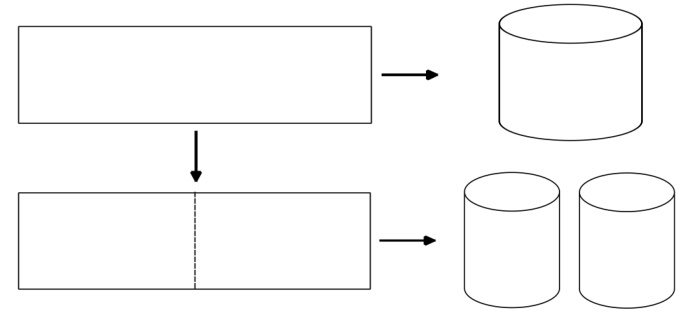
\includegraphics[scale =0.4]{toan05}
\end{center}
}{
\datcot
\bonpa
{\sai {$\dfrac{V_1}{V_2}=\dfrac{1}{2}$.}}
{\sai {$\dfrac{V_1}{V_2}=1$.}}
{\dung{$\dfrac{V_1}{V_2}=2$.}}
{\sai {$\dfrac{V_1}{V_2}=4$.}}
\loigiai{
Một đường tròn có bán kính r thì có chu vi và diện tích lần lượt là $C=2\pi t; S=\pi r^2\Rightarrow S=\dfrac{C^2}{4\pi}$.\\
Gọi chiều dài tấm tôn là a thì tổng diện tích đáy của thùng theo 2 cách lần lượt là\\
$S_1=\dfrac{a^2}{4\pi}; S_2=2.\dfrac{\left(\tfrac{a}{2}\right)}{4\pi}=\dfrac{a^2}{8\pi}\Rightarrow \dfrac{S_1}{S_2}=2\Rightarrow \dfrac{V_1}{V_2}=2$.
}  
}

\baitracnghiem{t2017:b41}{%
Trong không gian, cho hình chữ nhật $ABCD$ có $AB = 1$ và $AD = 2.$ Gọi $M, N$
lần lượt là trung điểm của $AD$ và $BC$. Quay hình chữ nhật đó xung quanh trục $MN$, ta
được một hình trụ. Tính diện tích toàn phần $S_{tp} $ của hình trụ đó.
}{
\datcot
\bonpa
{\dung{$S_{tp}=4\pi$.}}
{\sai {$S_{tp}=2\pi$.}}
{\sai {$S_{tp}=6\pi$.}}
{\sai {$S_{tp}=10\pi$.}}
\loigiai{
Hình trụ có bán kính đáy $r = 1$, chiều cao $h = 1$ nên có $S_{\varphi}=2\pi r^2+2\pi r h=4\pi$. 
}  
}

\baitracnghiem{t2017:b42}{%
Cho hình chóp $S.ABC$ có đáy $ABC$ là tam giác đều cạnh bằng 1, mặt bên $SAB$ là
tam giác đều và nằm trong mặt phẳng vuông góc với mặt phẳng đáy. Tính thể tích $V$ của
khối cầu ngoại tiếp hình chóp đã cho.
}{
\datcot
\bonpa
{\sai {$V=\dfrac{5\sqrt{15}\pi}{18}$.}}
{\dung{$V=\dfrac{5\sqrt{15}\pi}{54}$.}}
{\sai {$V=\dfrac{4\sqrt{3}\pi}{27}$.}}
{\sai {$V=\dfrac{5\pi}{3}$.}}
\loigiai{
Gọi $M,N,P,Q$ lần lượt là trung điểm $AB$, tâm đường tròn ngoại tiếp $\Delta SAB$, tâm cầu ngoại tiếp
chóp và tâm đường tròn ngoại tiếp $\Delta SBC$ $\Rightarrow MNPQ$ là hình vuông suy ra\\
$PN=MQ=\dfrac{1}{3}.\dfrac{\sqrt3}{2}=\dfrac{\sqrt3}{6}; NB=\dfrac{2}{3}.\dfrac{\sqrt3}{2}=\dfrac{\sqrt3}{3}$.\\
Bán kính hình cầu ngoại tiếp chóp là  $R=PB=\sqrt{PN^2+NB^2}=\dfrac{\sqrt{15}}{6}$.\\
Thể tích $V=\dfrac{4}{3}\pi R^3= \dfrac{5\sqrt{15}\pi}{54}$. 
}  
}

\baitracnghiem{t2017:b43}{%
Trong không gian với hệ tọa độ $Oxyz$, cho mặt phẳng $(P) : 3x - z + 2 = 0$. Vectơ
nào dưới đây là một vectơ pháp tuyến của (P) ?
}{
\datcot
\bonpa
{\sai {$\overrightarrow{n_4}=(-1;0;-1)$.}}
{\sai {$\overrightarrow{n_1}=(3;-1;2)$.}}
{\sai {$\overrightarrow{n_3}=(3;-1;0)$.}}
{\dung{$\overrightarrow{n_2}=(3;0;-1)$.}}
\loigiai{
Có (P): $3x + 0y - z + 2 = 0$ nên $(3;0;-1)$ là 1 VTPT của (P). Chọn D.
}  
}

\baitracnghiem{t2017:b44}{%
Trong không gian với hệ tọa độ $Oxyz$, cho mặt cầu
$$(S):(x+1)^2+(y-2)^2+(z-1)^2=9.$$
Tìm tọa độ tâm $I$ và tính bán kính $R$ của $(S)$.
}{
\datcot[2]
\bonpa
{\dung{$I(-1;2;1)$ và $R=3$.}}
{\sai {$I(1;-2;-1)$ và $R=3$.}}
{\sai {$I(-1;2;1)$ và $R=9$.}}
{\sai {$I(1;-2;-1)$ và $R=9$.}}
\loigiai{
$I(-1;2;1)$ và $R=3$.
}  
}
% 
\baitracnghiem{t2017:b45}{%
Trong không gian với hệ tọa độ $Oxyz$, cho mặt phẳng $(P) $:  
$3x+4y+2z+4=0$
và điểm $A(1; -2; 3).$ Tính khoảng cách $d$ từ $A$ đến ($P$).
}{
\datcot
\bonpa
{\sai {$d=\dfrac{5}{9}$.}}
{\sai {$d=\dfrac{5}{29}$.}}
{\dung{$d=\dfrac{5}{\sqrt{29}}$.}}
{\sai {$d=\dfrac{\sqrt5}{3}$.}}
\loigiai{
$d(A;(P))=\dfrac{|3.1+4.(-2)+2.3+4|}{\sqrt{3^2+4^2+2^2}}
=\dfrac{5}{\sqrt{29}}$.
}  
}

\baitracnghiem{t2017:b46}{%
Trong không gian với hệ tọa độ $Oxyz$, cho đường thẳng $\Delta$ có phương trình :
$$\dfrac{x-10}{5}=\dfrac{y-2}{1}=\dfrac{z+2}{1}.$$
Xét mặt phẳng $(P) : 10x + 2y + mz + 11 = 0$, $m$ là tham số thực. Tìm tất cả các giá trị của
$m$ để mặt phẳng ($P$) vuông góc với đường thẳng $\Delta$.
}{
\datcot
\bonpa
{\sai {$m=-2$.}}
{\dung{$m=2$.}}
{\sai {$m=-52$.}}
{\sai {$m=52$.}}
\loigiai{
Đường thẳng $\Delta$ nhận $(5;1;1)$ là 1 VTCP.
(P) nhận $(10;2;m)$ là 1 VTPT.\\
$(d)\perp (P)\Leftrightarrow (10;2;m)=k.(5;1;1)\Leftrightarrow k=2$ và $m=2$. 
}  
}

\baitracnghiem{t2017:b47}{%
Trong không gian với hệ tọa độ $Oxyz$, cho hai điểm $A(0; 1; 1)$ và $B(1; 2; 3)$.
Viết phương trình của mặt phẳng $(P)$ đi qua $A$ và vuông góc với đường thẳng $AB$.
}{
\datcot[2]
\bonpa
{\dung{$x + y + 2z - 3 = 0$.}}
{\sai {$x + y + 2z - 6 = 0$.}}
{\sai {$x + 3y + 4z -7 = 0$.}}
{\sai {$ x + 3y + 4z - 26 = 0$.}}
\loigiai{
(P) nhận   $\overrightarrow{AB}=(1;1;2)$ làm VTPT. (P) qua $A\Rightarrow$ (P): $x+y-1+2(z-1)=0\Leftrightarrow x+y+2z-3=0$. 
}  
}

\baitracnghiem{t2017:b48}{%
Trong không gian với hệ tọa độ $Oxyz$, cho mặt cầu ($S$) có tâm $I(2; 1; 1)$ và mặt
phẳng $(P) :$  $2x+y+2z+2=0$. Biết mặt phẳng ($P$) cắt mặt cầu ($S$) theo giao tuyến là
một đường tròn có bán kính bằng 1. Viết phương trình của mặt cầu ($S$).
}{
\datcot[2]
\bonpa
{\sai {$(S)$: $(x+2)^2+(y+1)^2+(z+1)^2=8$.}}
{\sai {$(S)$: $(x+2)^2+(y+1)^2+(z+1)^2=10$.}}
{\sai {$(S)$: $(x-2)^2+(y-1)^2+(z-1)^2=8$.}}
{\dung{$(S)$: $(x-2)^2+(y-1)^2+(z-1)^2=10$.}}
\loigiai{
Có $d=d(I;(P))=\dfrac{|2.2+1+2.1+2|}{\sqrt{2^2+1^2+2^2}}=3$.\\
Bán kính mặt cầu là $R=\sqrt{d^2+1^2}=\sqrt{10}\Rightarrow (S): (x-2)^2+(y-1)^2=10$. 
}  
}

\baitracnghiem{t2017:b49}{%
Trong không gian với hệ tọa độ $Oxyz$, cho điểm $A(1; 0; 2)$ và đường thẳng $d$ có
phương trình : $\dfrac{x-1}{1}=\dfrac{y}{1}=\dfrac{z+1}{2}$.
Viết phương trình đường thẳng $\Delta$ đi qua $A$, vuông
góc và cắt $d$.
}{
\datcot[2]
\bonpa
{\sai {$\Delta$: $\dfrac{x-1}{1}=\dfrac{y}{1}=\dfrac{z+2}{1}$.}}
{\dung{$\Delta$: $\dfrac{x-1}{1}=\dfrac{y}{1}=\dfrac{z+2}{-1}$.}}
{\sai {$\Delta$: $\dfrac{x-1}{2}=\dfrac{y}{2}=\dfrac{z-2}{1}$.}}
{\sai {$\Delta$: $\dfrac{x-1}{1}=\dfrac{y}{-3}=\dfrac{z-2}{1}$.}}
\loigiai{ 
Phương trình mặt phẳng qua $A$ và vuông góc (d): \\
$(x - 1) + y + 2(z - 2) = 0 \Leftrightarrow x+y+2z-5=0$ (P). Giao d và (P) là $B(2;1;1)$.\\
Phương trình đường thẳng cần tìm là $AB$: $\dfrac{x-1}{1}=\dfrac{y}{1}=\dfrac{z-2}{-1}$. 
}  
}

\baitracnghiem{t2017:b50}{%
Trong không gian với hệ tọa độ $Oxyz$, cho bốn điểm $A(1; -2; 0), B(0; -1; 1)$,
$C(2; 1; -1)$ và $D(3; 1; 4)$. Hỏi có tất cả bao nhiêu mặt phẳng cách đều bốn điểm đó ?
}{
\datcot[2]
\bonpa
{\sai {1 mặt phẳng.}}
{\sai {4 mặt phẳng.}}
{\dung{7 mặt phẳng.}}
{\sai {Có vô số mặt phẳng.}}
\loigiai{
Ta có phương trình mặt phẳng $(ABC): x + z - 1 = 0$\\
$\Rightarrow D\not\in (ABC)\Rightarrow 4$ $A, B, C, D$ không đồng phẳng.\\
Gọi (P) là mặt phẳng cách đều 4 điểm $A, B, C, D$: Có 2 trường hợp\\
+ Có 1 điểm nằm khác phía với 3 điểm còn lại so với mặt phẳng (P): Có 4 mặt phẳng (P) thỏa
mãn.\\
+ Mỗi phía của mặt phẳng (P) có 2 điểm: Có 3 mặt phẳng (P) thỏa mãn.\\
Vậy có 7 mặt phẳng thỏa mãn.
}  
}
